\BiChapter{马尔可夫链蒙特卡罗方法}{MCMC}
蒙特卡罗方法被评为“20世纪十大算法”之一,自20世纪50年代该方法被提出后的几十年里已被学术界与工业界广泛应用。这套方法最初源自于Stan Ulam对纸牌游戏的思考,他试图计算52张卡牌的组合可能,在尝试穷举失败后,他意识到需要一种随机方法去求取近似解而不是花费大量时间求取一个精确解。随后,他找到冯·诺依曼,两人共同完善了蒙特卡罗方法的一些理论,比如重要性采样和舍弃采样。由于蒙特卡罗方法是一整套解决方案,算法众多,其理论贡献不能仅仅归功于这两人,还应包括提出MH算法的Metroplis和Hasting、将蒙特卡罗方法应用到中子扩散问题的Fermi等。20世纪80年代,蒙特卡罗方法被引入机器视觉与人工智能领域,同时,在此之上加入马尔可夫链形成一套新的理论体系。这套理论常用于贝叶斯推断的归一化、边缘化与期望问题,概率论的配分函数问题,最优化问题以及机器学习中的模型选择问题。



\BiSection{蒙塔卡罗方法核心思想\label{section:MCidea}}
x蒙特卡罗方法的一个应用是计算一个分布下某个函数的期望,现在假设我们要计算一个积分
\begin{equation}\label{equ:int}
I_f = \int_{-\infty}^{+\infty} (2x^2 + x + 1) \frac{1}{\sqrt{2\pi}} \exp\Big(-\frac{1}{2}x^2\Big)dx
\end{equation}
为了简化,我们记
\begin{equation}\label{equ:f(x)}
f(x) = 2x^2 + x + 1
\end{equation}
\begin{equation}
p(x) = \frac{1}{\sqrt{2\pi}} \exp\Big(-\frac{1}{2}x^2\Big)
\end{equation}
那么,式\eqref{equ:int}可以简写为
\begin{equation}\label{equ:MCintFull}
I_f = \int_{-\infty}^{+\infty} f(x)\cdot p(x) dx
\end{equation}

由于$p(x)$恰好是一个标准高斯分布,倘若我们能从$p(x)$中采样得到$N$个独立同分布(i.i.d)样本$\{x_i\}_{i=1}^N$,则积分$I_f$可以近似为
\begin{equation}\label{equ:MCintProx}
I_f \approx \hat{I}_f = \frac{1}{N}\sum\limits_{i=1}^N f(x_i)
\end{equation}
此时,若$N\rightarrow \infty$,根据大数定律,可知
\begin{equation}
I_f = \lim\limits_{N\rightarrow \infty} \hat{I}_f = \lim\limits_{N\rightarrow \infty} \frac{1}{N}\sum\limits_{i=1}^N f(x_i)
\end{equation}

倘若从数学期望的角度上来解释上面的问题,那么积分\eqref{equ:int}可以理解为:我们现在有一个函数$f(x) = 2x^2 + x+ 1$,其自变量$x$符合标准高斯分布,即$x\sim \mathcal{N}(0, 1)$,那么为了计算$f(x)$在分布$\mathcal{N}(0, 1)$下的数学期望,我们可以在分布$\mathcal{N}(0, 1)$中采样出N个独立的样本$\{x_i\}_{i=1}^N$,将这些样本代入$f(x)$,得到$N$个函数值$\{f(x_i)\}_{i=1}^N$,对这些函数值求和取平均后得到的结果即为期望$I_f$的近似值$\hat{I}_f$。显然,其近似程度与$N$有关,$N$越大,采样的样本越多,近似的程度也便越高。

但积分\eqref{equ:int}未免过于特殊,首先,$p(x)$是一个标准高斯分布,这使得我们可以利用一些很成熟的方法来从$\mathcal{N}(0, 1)$中采样出$N$个样本,但如果$p(x)$不是一个高斯分布,也不是一个均匀分布、伽马分布等一些我们常见的概率分布,它只是一个普通得不能再普通的分布 ,此时又该如何解决?其次,积分\eqref{equ:int}只是一维形式,而实际生活中的概率分布往往是高维的,那么高维情况又该如何推广?接下来的几个小节我们将致力于解决以上几个问题。

\BiSection{舍弃采样}{rejectionSampling}
我们先来解决之前提到的第一个问题,如果说$p(x)$不是一个常见的概率分布应该如何解决?例如
\begin{equation}\label{equ:p(x)}
p(x) = 0.3 \frac{1}{\sqrt{2\pi}}\exp\Big(-\frac{(x-2)^2}{2}\Big) + 0.7 \frac{1}{\sqrt{2\pi}}\exp\Big(-\frac{(x+2)^2}{2}\Big)
\end{equation}
当$f(x)$依然设定为\eqref{equ:f(x)}时,概率密度曲线$p(x)$以及函数$f(x)\cdot p(x)$的图像如图\ref{img:pxAndfxpx} 所示
\begin{figure}[htbp]\label{img:pxAndfxpx}
\centering
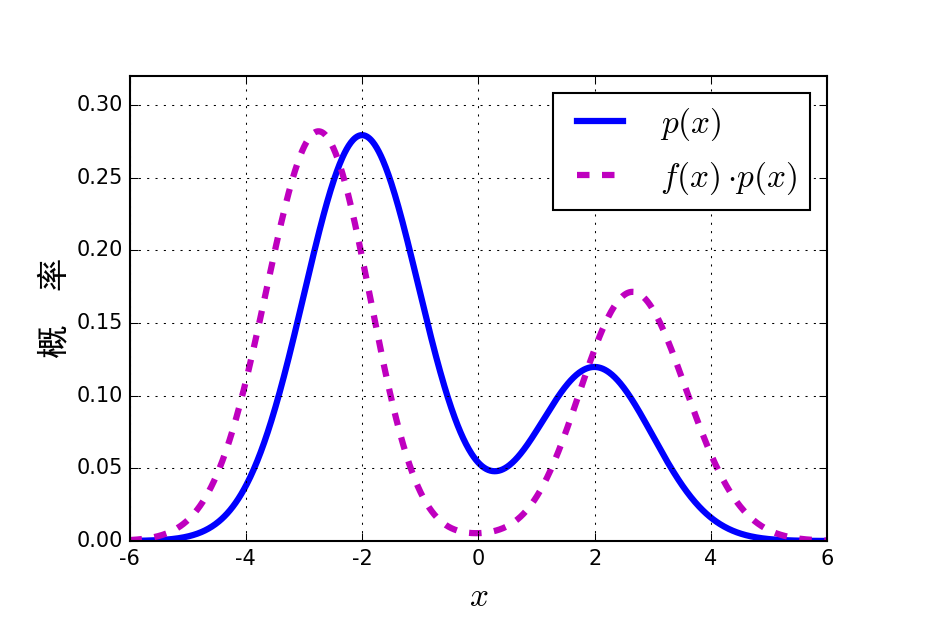
\includegraphics[width=0.5\textwidth]{MCMC/rejectionPxAndfxPx.eps}
\caption{实际分布$p(x)$与$f(x)\cdot p(x)$的函数图像}
\end{figure}

此时,由于$p(x)$并不是一个常见的概率分布,而我们所拥有的一些简单的采样方案基本都是针对于某一类特定的分布而提出的,基于这个原因,这里要想在$p(x)$中采样出$N$个样本并不是一件简单的工作。为此,我们引入舍弃采样来解决在任意分布上采样的问题。

舍弃采样基于这样一个思想:既然我们无法从一个随意的分布$p(x)$上采样,但是可以在一个特殊的分布$q(x)$上采样,比如从高斯分布中采样,那么我们为何不用$q(x)$来逼近$p(x)$呢?为此,我们引入一个分布$q(x)$,称之为提议分布,这个分布需要满足以下条件
\begin{equation}
p(x) < Mq(x),~~~~M<\infty
\end{equation}
式中,$M$是一个定常数,上述约束条件相当于,提议分布$q(x)$与实际分布$p(x)$的比值$p(x)/q(x)$需要在变量$x$的空间$\mathcal{X}$中存在下界$M$。从图像的角度看,提议分布扩大$M$倍后,应该“覆盖”,或者说“包着”实际分布$p(x)$,例如,对于式\eqref{equ:p(x)}的分布$p(x)$,当$M=2.3$且提议分布$q(x)$为
\begin{equation}\label{equ:q(x)}
q(x) = \frac{1}{3\sqrt{2\pi}}\exp\Big(-\frac{(x+1.3)^2}{2\times 3^2}\Big)
\end{equation}
即$q(x)\sim \mathcal{N}(-1.3, 3)$时,实际分布$p(x)$与提议分布$q(x)$的图像如图\ref{img:pxAndqx} 所示

\begin{figure}[htbp]\label{img:pxAndqx}
\centering
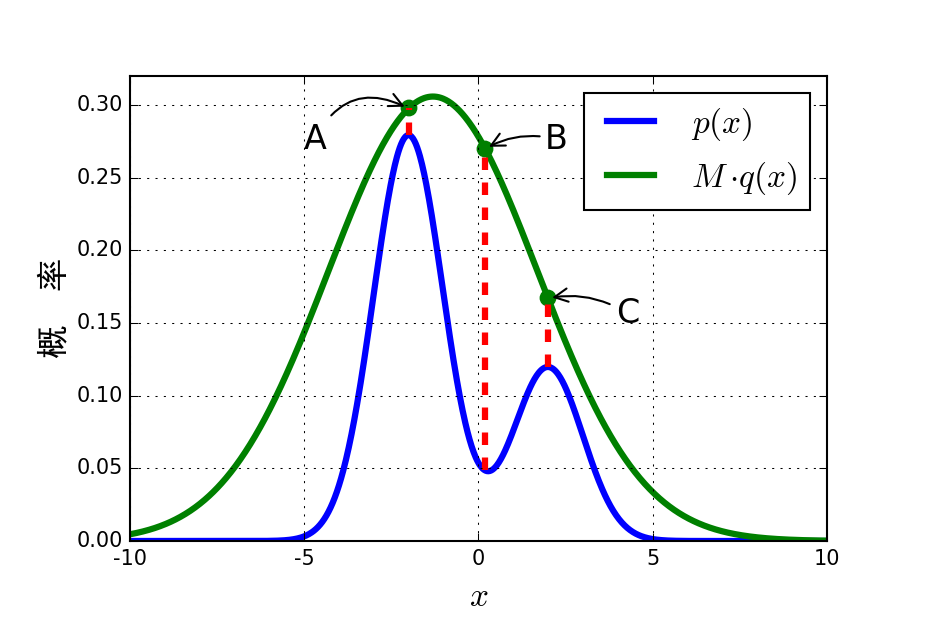
\includegraphics[width=0.5\textwidth]{MCMC/rejectionPxAndQx.eps}
\caption{实际分布$p(x)$与提议分布$q(x)$的函数图像}
\end{figure}

由于提议分布是一个常规的高斯分布,我们有一系列的成熟方法可以在其之上采样出多个样本。假设我们采样得到一个样本后,我们有两种选择:要么接受这个样本,并将这个样本看做是从$p(x)$上采样得到的,要么舍弃这个样本,认为这个样本与$p(x)$采样的样本差距太大,不能看做是$p(x)$的采样样本。

然而,我们什么时候应该接受$q(x)$的样本作为$p(x)$的样本,什么时候又应该拒绝呢?为了刻画这个事件,我们引入了接受概率的概念。假定我们现在已从$q(x)$中采样得到一个样本$x^{(i)}$,则其接受概率$A$我们定义为
\begin{equation}
A = \frac{p(x^{(i)})}{M\cdot q(x^{(i)})}
\end{equation}

计算得到接受概率后,我们以$A$作为接受样本的概率,但在计算机中,没有一种方法直接地描述“以概率A接受样本”这个行为,为了仿真这个行为,我们可以在区间为$[0, 1]$的均匀分布$U(0,1)$上随机生成一个数$u$,若$u<A$则接受样本,否则拒绝。通过这样的方式,我们便可以模拟“以A为概率接受样本”。我们很容易将一个样本推广到$N$个样本的情况,其具体描述如算法\ref{alg:rejection}所示。

\vspace{1em}
\begin{minipage}{0.8\textwidth}\centering
\begin{algorithm}[H]\label{alg:rejection}
 \caption{舍弃采样算法}
  \KwIn{真实分布$p(x)$;提议分布$q(x)$; 采样量$N$}
 \KwOut{$N$个采样样本$\{x^{(i)}\}_{i=1}^N$}
$i=1$\;
\Repeat{$i=N$}
{
采样$x^{(i)}\sim q(x)$,获取随机数$u\sim U(0,1)$,$A = \frac{p(x^{(i)})}{M\cdot q(x^{(i)})}$;\\
\If{$u<A$}
{
接受样本$x^{(i)}$作为$p(x)$的样本,$i += 1$;\\
}
\Else{舍弃样本$x^{(i)}$,$i$保持不变;}
}
\end{algorithm}
\end{minipage}
\vspace{1em}

对于接受概率其定义,一种较为直观的理解是:接受概率$A(x^{(i)})$刻画了$p(x^{(i)})$与$Mq(x^{(i)})$的相似程度。如图\ref{img:pxAndqx}中的A、B、C三点,假设我们可以分别从两个分布中采样得到多个样本,对于$q(x)$而言,采样样本出现在A点附近的概率最大,其次是B点附近,再次是C点附近。然而,对于$p(x)$而言,采样样本出现在B点附近的概率要比出现在C点附近的概率要小,因此,把从$q(x)$中采样得到的样本直接作为$p(x)$的采样样本是不合适的。但由于
\begin{equation}
\frac{p(x_{B\text{附近}})}{M\cdot q(x_{B\text{附近}})} < \frac{p(x_{C\text{附近}})}{M\cdot q(x_{C\text{附近}})}
\end{equation}
B点较小的接受概率使得我们舍弃了$q(x)$采样样本中B点附近大量的样本,C点较大的接受概率使得我们保留了$q(x)$采样样本中C点附近的大量样本,经过舍弃阶段后,我们便可以从$q(x)$的采样样本中筛选出可以刻画$p(x)$性质的样本,因此,舍弃操作可以看做是对样本的纠正。

在$q(x)$定义为式\eqref{equ:q(x)},$p(x)$定义为式\eqref{equ:p(x)}且$M=2.3$的情况下,图\ref{img:hist q(x)}为$q(x)$及采样样本的概率分布直方图,将这些样本经过舍弃后,其分布直方图如图\ref{img:hist P(x)}所示。不难看出,尽管样本是从提议分布$q(x)$中采样得到的,但舍弃采样方法可以很好地逼近原始分布,因此我们可以用筛选后的样本间接地作为$p(x)$的采样样本而不再需要从$p(x)$中直接采样。

\begin{figure}[htbp]
\centering
\subfigure{\label{img:hist q(x)}}\addtocounter{subfigure}{-2}
\subfigure{\subfigure[$q(x)$与样本分布直方图]
			{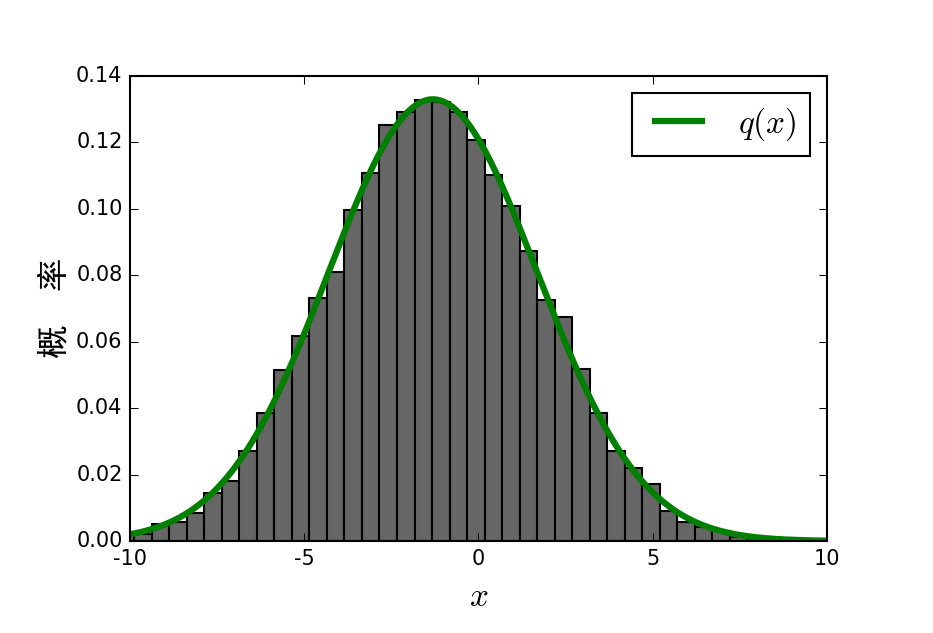
\includegraphics[width=0.4\textwidth]{MCMC/histQx.eps}}}
\subfigure{\label{img:hist P(x)}}\addtocounter{subfigure}{-2}
\subfigure{\subfigure[$p(x)$与筛选后的样本分布直方图]
			{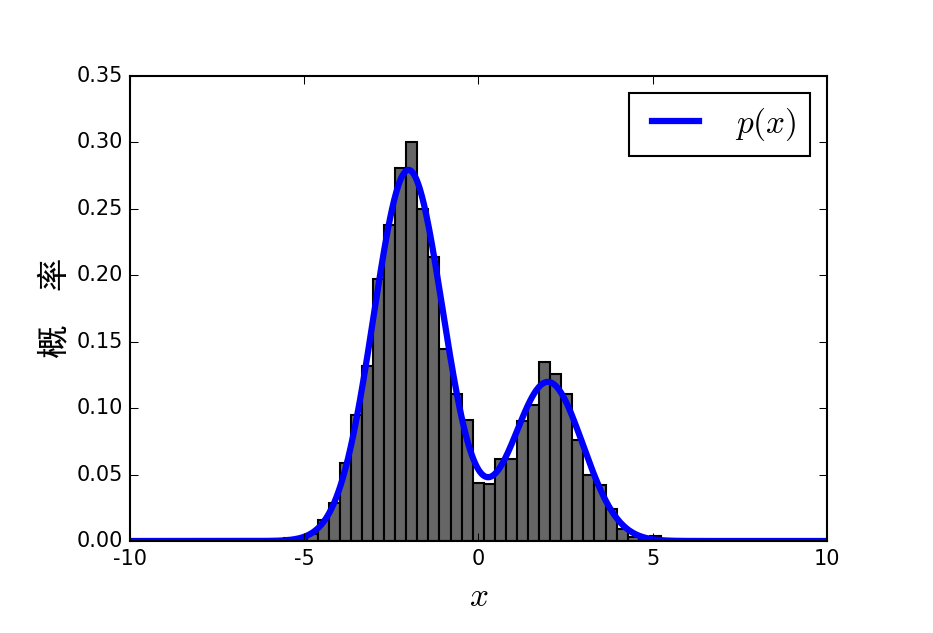
\includegraphics[width=0.4\textwidth]{MCMC/histPx.eps}}}
\caption{舍弃采样的逼近效果}
\vspace{-1em}
\end{figure}

事实上,式\eqref{equ:p(x)}依然过于特殊,其概率密度不过是两个一维高斯分布的线性组合,如果我们将其扩展到二维情形,例如,当真实分布$p(x)$与提议分布$q(x)$分别定义为
\begin{equation}
\begin{split}
p(x) =
& 0.2\cdot \frac{1}{2\pi} \exp\bigg(-\frac{(x+1)^2 + (y+1)^2}{2}\bigg)~ + \\
& 0.1\cdot \frac{1}{2\pi} \exp\bigg(-\frac{(x-3)^2 + (y+3)^2}{2}\bigg)~ +\\
& 0.7\cdot \frac{1}{2\pi} \exp\bigg(-\frac{(x-2)^2 + y^2}{2}\bigg) \\
\end{split}
\end{equation}
\begin{equation}
q(x) = \frac{1}{2\times 2^2 \cdot \pi} \exp\bigg(-\frac{(x-1.5)^2 + y^2}{2\times 2^2}\bigg)
\end{equation}
在$M = 3$时,真实分布与提议分布的图像如图\ref{img:2Dgaussian} 所示

\begin{figure}[htbp]
\centering
\subfigure{\label{img: 2Dgaussian full}}\addtocounter{subfigure}{-2}
\subfigure{\subfigure[全视图]
			{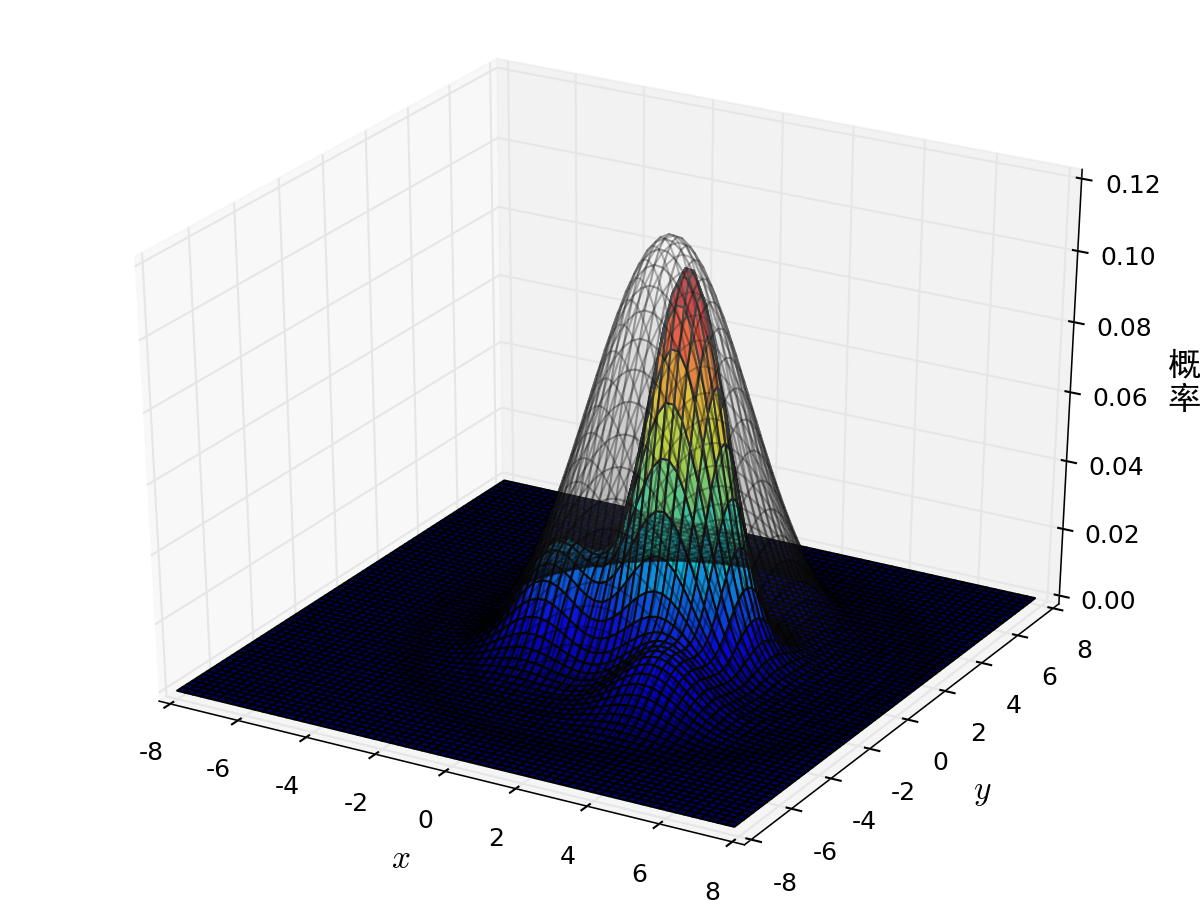
\includegraphics[width=0.4\textwidth]{MCMC/2Dgaussian.eps}}}
\subfigure{\label{img:2Dgaussian part}}\addtocounter{subfigure}{-2}
\subfigure{\subfigure[剖视图]
			{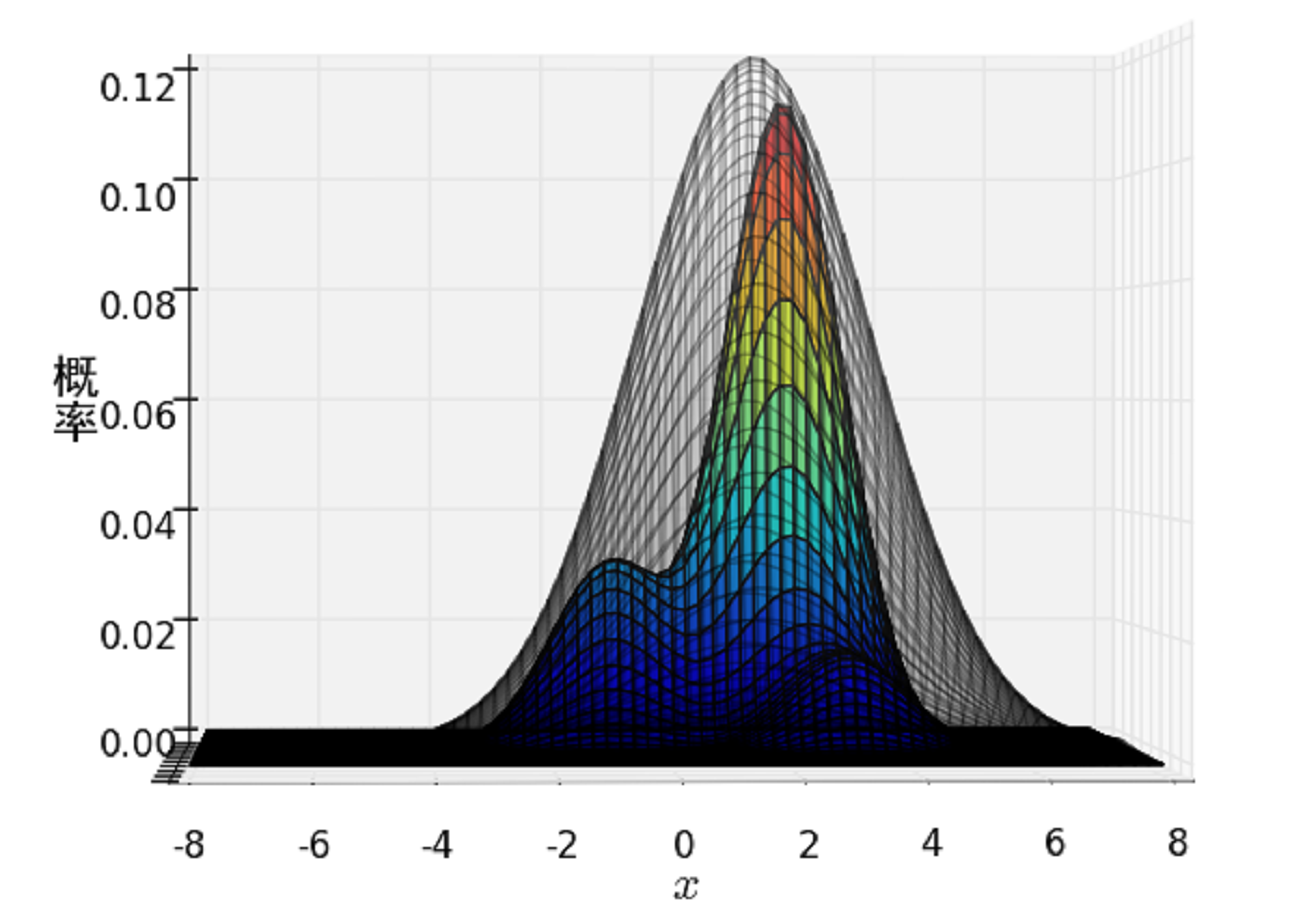
\includegraphics[width=0.4\textwidth]{MCMC/2DgaussianPart.eps}}}
\caption{二维真实分布(彩色)与提议分布(灰色)}
\label{img:2Dgaussian}
\vspace{-1em}
\end{figure}

以上例子都过于简单,实际中我们遇到的一般都是高维的情形,概率密度也更为复杂。这将会导致一个结果,提议分布$q(x)$为了“包住”真实分布$p(x)$,$M$需要取一个很大的值使得$q(x)$可以覆盖掉最凸出的维度。想象这样一种极端的情形,在一个高维度的$p(x)$中,有一个维度是类似于脉冲的尖峰,此时$M$需要取很大才足以覆盖它,但对于剩余的维度而言,$M$可能只需要一个较小的值便可以覆盖掉它们,为了使约束$p(x)< M\cdot q(x)$恒成立,M需要取最大的值,过大的$M$使得接受概率$A = p(x)/Mq(x)$过小,大规模地舍弃样本将使采样速度变慢甚至无法再可以接受的时间内完成采样。究其原因,其最根本的弊端在于$q(x)$必须满足约束$p(x)< M\cdot q(x)$。为了解决这个问题,我们将引入重要性采样,这种方法可以使我们不受约束地选取任意的$q(x)$。


\BiSection{重要性采样}
x回顾章节\ref{section:MCidea}中的讨论,我们为什么要使用舍弃采样?因为蒙特卡罗方法中积分式\eqref{equ:MCintFull}在$p(x)$不是常规的分布形式时难以采样,导致我们无法利用式\eqref{equ:MCintProx}来计算积分。而舍弃采样通过构建一个容易采样的分布$q(x)$,对其采样样本筛选后作为$p(x)$的样本,式\eqref{equ:MCintProx}从而得以进行下去。

式\eqref{equ:MCintProx}之所以能成立,是因为我们利用了点质量函数来逼近概率密度,即
\begin{equation}\label{equ:pn}
p_N(x) = \frac{1}{N}\sum\limits_{i=1}^N \delta_{x^{(i)}}(x)
\end{equation}
式中,$\delta_{x^{(i)}}(x)$为$x^{(i)}$处的脉冲函数。倘若我们不采用这种逼近方式,而采用另外一种,在介绍这种方式之前,我们先引入所谓的重要性权值$w(x)$,即
\begin{equation}
w(x) = \frac{p(x)}{q(x)}
\end{equation}
式中,$q(x)$为任意一个分布。此时,新的逼近方式可以陈述为
\begin{equation}
\hat{p}_N(x) = \sum\limits_{i=1}^N w(x^{(i)})\delta_{x^{(i)}}(x)
\end{equation}
对比式\eqref{equ:pn},我们可以理解为$p_N(x)$中的$1/N$相当于重要性权值恒为$1/N$。引入重要性权值后,积分式\eqref{equ:MCintFull}可以改写为
\begin{equation}
I_f = \int_{-\infty}^{+\infty} f(x)w(x)q(x) dx
\end{equation}
对应的,式\eqref{equ:MCintProx}改写为
\begin{equation}
\hat{I}_f \approx \sum\limits_{i=1}^N f(x^{(i)}) w(x^{(i)})
\end{equation}

如果从另一个角度思考,以上讨论相当于,我们现在有一个目标函数$f(x)$及概率分布$p(x)$,要计算$f(x)$在分布$p(x)$下的期望,由于$p(x)$不是一个常见的分布形式,导致难以利用式\eqref{equ:MCintProx}计算积分, 那么我们构建一个常见的分布形式$q(x)$,将目标函数改写为
\begin{equation}
\hat{f}(x) = \frac{f(x)p(x)}{q(x)} = f(x)w(x)
\end{equation}
则积分式\eqref{equ:MCintFull}变为
\begin{equation}
\hat{I}_f =  \int_{-\infty}^{+\infty} \hat{f}(x)q(x) dx
\end{equation}
此时我们又可以使用类似于式\eqref{equ:MCintProx}的方式来计算积分了。

对比与之前讨论的舍弃采样而言,重要性采样的优点在于$q(x)$不受约束,也不存在舍弃行为,这使得算法效率相对与舍弃采样有所提高。但重要性采样也有其内在缺点,即$q(x)$选取的好坏程度影响着积分的精度,若$q(x)$选取得不好,则需要大量的样本来提高积分精度。刻画$q(x)$好坏的一种准则是最小化$\hat{I}_N f(x)$的方差,即
\begin{equation}
var_{q(x)}\Big[f(x)w(x)\Big] = \mathbb{E}\Big[f^2(x)w^2(x)\Big] - I^2(f)
\end{equation}
由于$I^2(f)$于$q(x)$无关可以摄取,再利用Jensen不等式,有
\begin{equation}
\mathbb{E}\Big[f^2(x)w^2(x)\Big] \geq \mathbb{E}^2\Big[|f(x)|w(x)\Big] = \Big(\int |f(x)|p(x)dx\Big)^2
\end{equation}
因此提议分布可以选取为
\begin{equation}
q(x) = \frac{|f(x)|p(x)}{\int |f(x)|p(x)dx}
\end{equation}
由于分母只是一个归一化常数可以不管,我们现在要做的是在$|f(x)|p(x)$中采样,这看起来似乎没有什么用,实际上也确实没有什么用,毕竟$|f(x)|p(x)$并不似一个容易采样的函数。但它启示我们一点,如果$p(x)$的样本落在的重要域可以使得$|f(x)|p(x)$取值较大,那么采样效率将会非常高,这也是重要性采样的命名来源。

无论是舍弃采样还是重要性采样都是独立采样,即样本之间是独立的,从而采样效率较低。为了提高采样效率,我们可以使用关联采样,即样本之间存在关联,构建样本之间的关联性所要用到的便是著名的马尔可夫链。


\BiSection{马尔可夫链}
在正式引入马尔可夫链之前,我们打算先从一个随机游走的例子入手。想象一个正方形区域内,在某一点放入N个粒子,这些例子随机地朝着各个方向游走。对于每一个粒子而言,每一次游走的步长是相等的,只是角度随机选择。当粒子移动到正方形的边界是,它将被反弹回正方形区域内。直觉上的想象,经过漫长的时间,粒子将漫布在整个正方形区域内。如图\ref{img:randomWalk} 所示是两个随机游走的例子,其中蓝色的初始状态在中心附近,绿色的初始状态在左下角。
\begin{figure}[htbp]
\centering
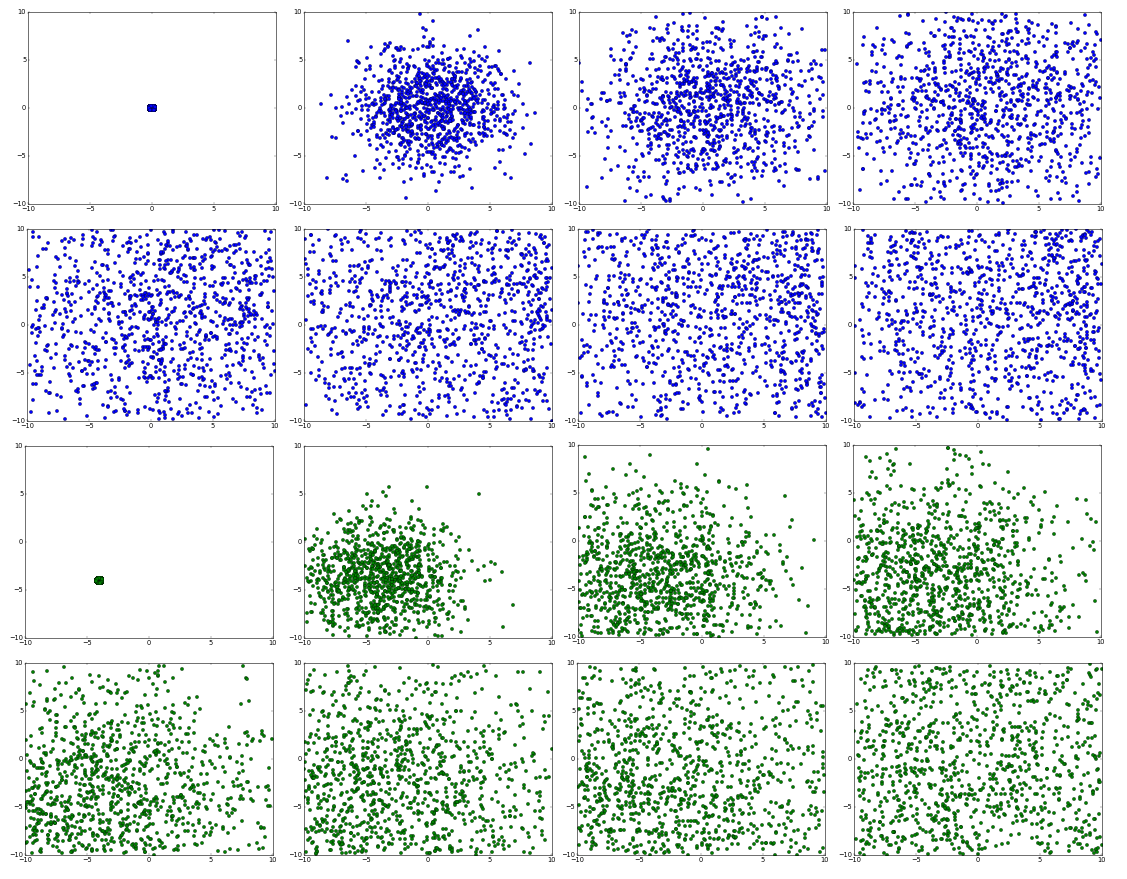
\includegraphics[width=0.5\textwidth]{MCMC/randomWalk.eps}
\caption{两个随机游走的例子}\label{img:randomWalk}
\end{figure}

这个例子类似于布朗运动,有趣的现象是,起始位置的选取并不会影响最终结果---粒子将呈均匀分布。正如一锅未加盐的汤,无论盐从哪个位置撒下,最终整锅汤的咸淡是均匀的。对于某个特定的粒子而言,追中它的轨迹是无意义的,从宏观上看,粒子下一步处于哪个位置与之前的位置无关,只与它当前的位置有关,因为它是经过怎样的路径到达当前的状态对下一步移动到哪里起不到任何作用。

马尔可夫链意识基于同一个原理,假设我们的变量$x$可取得状态有$s$个,那么集合$S = \{x_1, x_2, x_s\}$被称为状态空间,马尔可夫链刻画的是变量$x$在状态空间$S$中各个状态之间迁移的轨迹。类似于随机游走的例子,马尔可夫链的下一个状态与之前的状态无关,之与当前的状态有关,即
\begin{equation}
p(x^{(i+1)} | x^{(i)} \cdots x^{(1)}) = p(x^{(i+1)} | x^{(i)})
\end{equation}
这个性质也被称为马尔科夫性质。对于给定的系统,我们定义某个状态转移到另一个状态的概率为转移概率,即
\begin{equation}
p(x^{(i+1)} | x^{(i)}) = T(x^{(i)} \rightarrow x^{(i+1)})
\end{equation}

如图\ref{img:MCfigure} 中的系统,状态空间为$\{A, B, C\}$,由图中的参数我们容易算得转移矩阵$\mathcal{T}$
\begin{figure}[htbp]
\centering
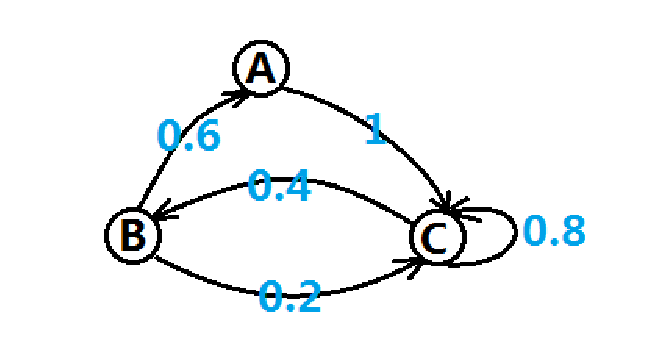
\includegraphics[width=0.5\textwidth]{MCMC/MCfigure.eps}
\caption{马尔科夫链}\label{img:MCfigure}
\end{figure}
\begin{equation}
\mathcal{T} = \left[
\begin{array}{ccc}
T(A\rightarrow A)~~ & T(A\rightarrow B)~~ & T(A\rightarrow C)\\
T(B\rightarrow A)~~ & T(B\rightarrow B)~~ & T(B\rightarrow C)\\
T(C\rightarrow A)~~ & T(C\rightarrow B)~~ & T(C\rightarrow C)\\
\end{array}
\right]
=\left[
\begin{array}{ccc}
0 & 0 & 1\\
0.6 &0 & 0.4\\
0 & 0.2 & 0.8
\end{array}
\right]
\end{equation}

倘若我们为A、B、C赋予一些实际意义,我们令A代表下雨,B代表多云,C代表晴天,又假设今天的天气为晴天,现在我们要估计10天后的天气状况。首先,我们可以很容易地将今天的天气描述为一个向量
\begin{equation}
x = [1~~0~~0]
\end{equation}
为了计算10天后的天气,用$x$乘以10次转移矩阵后将得到10天后的天气状况,即
\begin{equation}
[1~~0~~0] \times
\left[
\begin{array}{ccc}
0 & 0 & 1\\
0.6 &0 & 0.4\\
0 & 0.2 & 0.8
\end{array}
\right]^{10}
=[0.091~~0.151~~0.758]
\end{equation}
也就是说,10天后下雨的概率为0.091,多云的概率为0.151,晴天的概率为0.758。倘若我们假设今天的天气为多云,利用同样的方法,我们可以计算得10天后的天气状况为
\begin{equation}
[0~~1~~0] \times
\left[
\begin{array}{ccc}
0 & 0 & 1\\
0.6 &0 & 0.4\\
0 & 0.2 & 0.8
\end{array}
\right]^{10}
=[0.091~~0.151~~0.758]
\end{equation}
我们发现,不管今天是雨天开始多云,计算得到10天后的天气情况是十分接近的(这里完全一样是因为我们舍去了尾部小数),如果读者有兴趣的话可以验证初始状态为晴天是得到的结果也是一样的。也就是说,不管今天的天气如何,对10天后的天气均无影响。

之所以出现这种现象是因为马尔可夫链在第十个周期时已经进入一个我们称之为平稳的状态。类似于之前的随机游走,当经过足够长的时间后,系统的状态与初始状态再无关联,至于系统的结构(也就是转移矩阵)有关。但并不是所有的转移矩阵都能达到平稳,在这里,我们并不打算深入讨论,只给出结论定理
\begin{theorem}\label{theo:MC}
如果一个马尔科夫链是各态遍历的,那么存在一个时间$t_s$,当$t>t_s$时,马尔可夫链到达一个平稳分布$x^*$,其中$x^*$满足
\begin{equation}
x^* = x^* \mathcal{T}
\end{equation}
\end{theorem}
所谓各态遍历,即要求马尔可夫链是不可约且非周期的,所谓不可约,即所有状态都是有关联的,从某个状态出发,不存在无法到达的状态,所谓非周期,即马尔可夫链不会陷入某几个状态间循环,满足上述两个条件的马尔可夫链我们称它是各态遍历的。

利用马尔可夫链的这个性质,我们就可以实现关联采样。由于初始状态与稳态无关,我们可以随机设置,经过多次随机游走,进入稳态后得到的状态便可以作为一个样本。以上讨论均基于一个前提,即转移矩阵是已知的。然而,实际中,我们并不知道转移矩阵的数值。例如,我们并不知道由晴天转移到多云的概率是0.2,这个数值是我们捏造的。但是一旦转移矩阵知道了,采样问题便迎刃而解,目前成熟的马尔可夫链蒙特卡罗方法整体框架都是类似的,不同的地方往往在于转移矩阵的构造上。

\BiSection{Metropolis-Hastings算法}
x与舍弃采样类似,Metropolis-Hastings算法(以下简称MH算法)也存在一个提议分布,这个提议分布定义为$q(x^*|x)$,不同的是,舍弃采样中的提议分布受一个强约束,即$p(x) < Mq(x)$,而MH算法中的提议分布只需要满足$q(x^*|x)>0$即可,显然这个约束相当于没有约束,因为概率论三大公理的第一条就使这个约束成立了。另一个不同点在于,MH算法中的提议分布其意义为:在当前状态$x$下,由提议分布$q(x^*|x)$产生一个试探性状态$x^*$,随后根据接受概率决定是否转移到新状态$x^*$上,这里,接受概率定义为
\begin{equation}\label{equ:MHaccept}
A = \frac{p(x^*)\cdot q(x|x^*)}{p(x)\cdot q(x^*|x)}
\end{equation}
此时,若接受概率$A > 1$,则接受这个新状态,否则,以概率$A$接受新状态。若接受了这个新状态$x^*$,则状态从$x$转移到$x^*$处,并在$x^*$处的提议分布$q(x^{**}|x^*)$产生一个新的试探状态$x^{**}$,如此反复循环,若不接受这个状态$x^*$,则状态仍然停留$x$处。

需要注意的一点是,在MH采样中,提议分布$q(x^*|x)$是对着状态$x$的变动而变动的,例如,如果我们将提议分布$q(x^*|x)$设计成一个在以$x$为中心,以2为方差的高斯分布,即$q(x*|x)\sim \mathcal{N}(x, 2)$,那么如图\ref{img:diffStateDiffQx}所示,在$x^{(1)}$状态和$x^{(2)}$状态下的提议分布是不同的。

\begin{figure}[htbp]
\centering
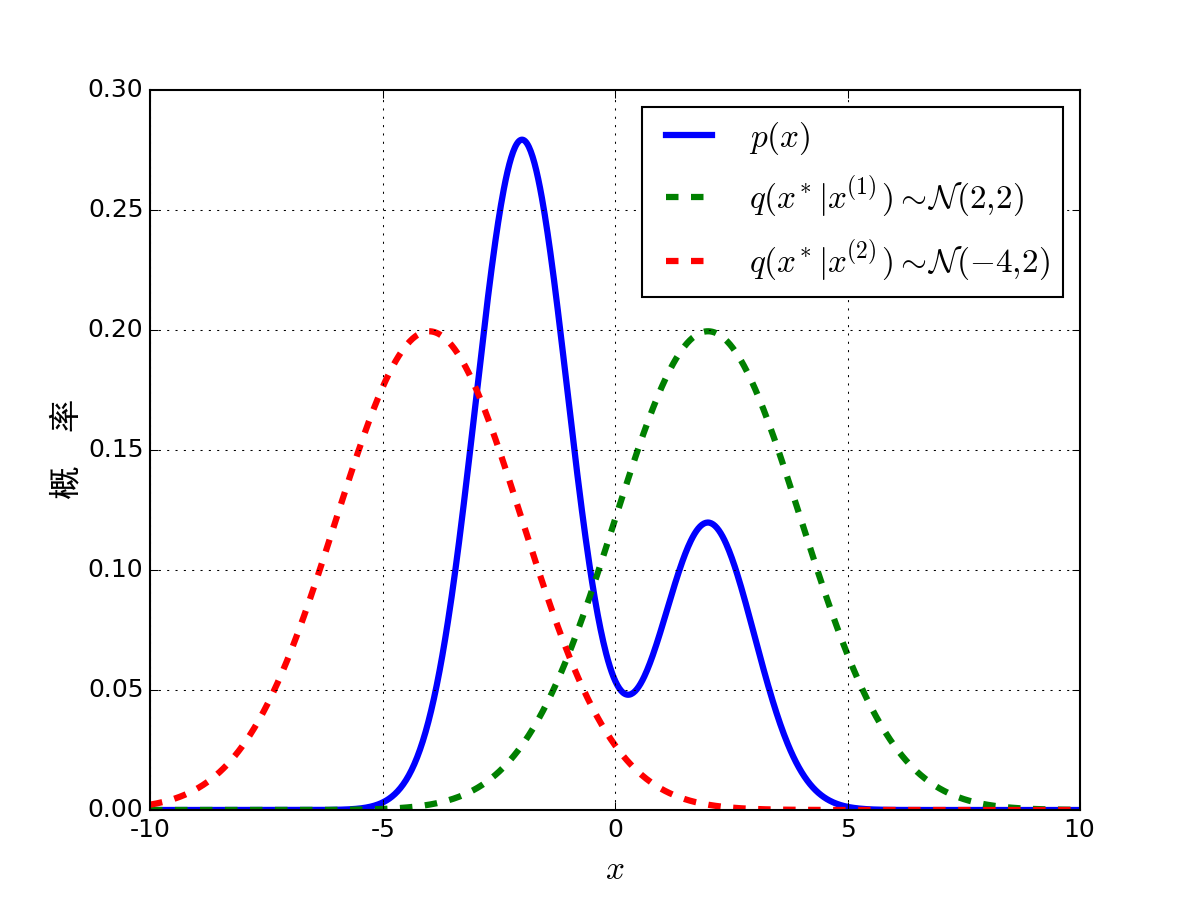
\includegraphics[width=0.5\textwidth]{MCMC/diffStateDiffQx.eps}
\caption{不同状态下的提议分布}\label{img:diffStateDiffQx}
\end{figure}


综合以上的讨论,MH算法可以描述为算法\ref{alg:MH} 中的过程。

\vspace{1em}
\begin{minipage}{0.8\textwidth}\centering
\begin{algorithm}[H]\label{alg:MH}
 \caption{Metropolis-Hastings算法}
  \KwIn{真实分布$p(x)$;提议分布$q(x^*|x)$; 游走次数$N$}
 \KwOut{$1$个采样样本$x^{(N)}$}
设置初始状态$x^{(0)}$,$i=0$\;
\Repeat{$i=N$}
{
采样$x^*\sim q(x^*|x^{(i)})$,获取随机数$u\sim U(0,1)$;\\
计算接受概率$A = \frac{p(x^*)\cdot q(x|x^*)}{p(x)q(x^*|x)}$\\
\If{$u<A$}
{
$x^{(i+1)} = x^*$;\\
}
\Else{$x^{(i+1)} = x^{(i)}$}
}
返回$x^{(N)}$
\end{algorithm}
\end{minipage}
\vspace{1em}

相比于舍弃采样,舍弃采样的拒绝是直接抛弃样本,而MH采样的拒绝是让样本停留在当前状态。另一个不同点在于,算法\ref{alg:MH}描述的是采样出一个样本的过程,是一个随机游走的过程,而算法\ref{alg:rejection}描述的是采样出$N$个样本的过程。尽管算法\ref{alg:MH}只能采样出一个样本,但是我们也可以很容易将其扩展成为残阳$N$个样本的算法。另外,由于各个样本的随机游走是独立的,不存在线程安全问题,因此算法\ref{alg:MH}可以很容易设计成为并行算法。

正如我们提到的,如果我们使用一个形式为$q(x*|x)\sim \mathcal{N}(x, 2)$的提议分布区采样1000个式\eqref{equ:p(x)}中实际分布$p(x)$的样本,对于不同的游走次数$N$,其结果如图\ref{img:MH} 所示

\begin{figure}[htbp]
\centering
\subfigure{}\addtocounter{subfigure}{-2}
\subfigure{\subfigure[$N=10$]
			{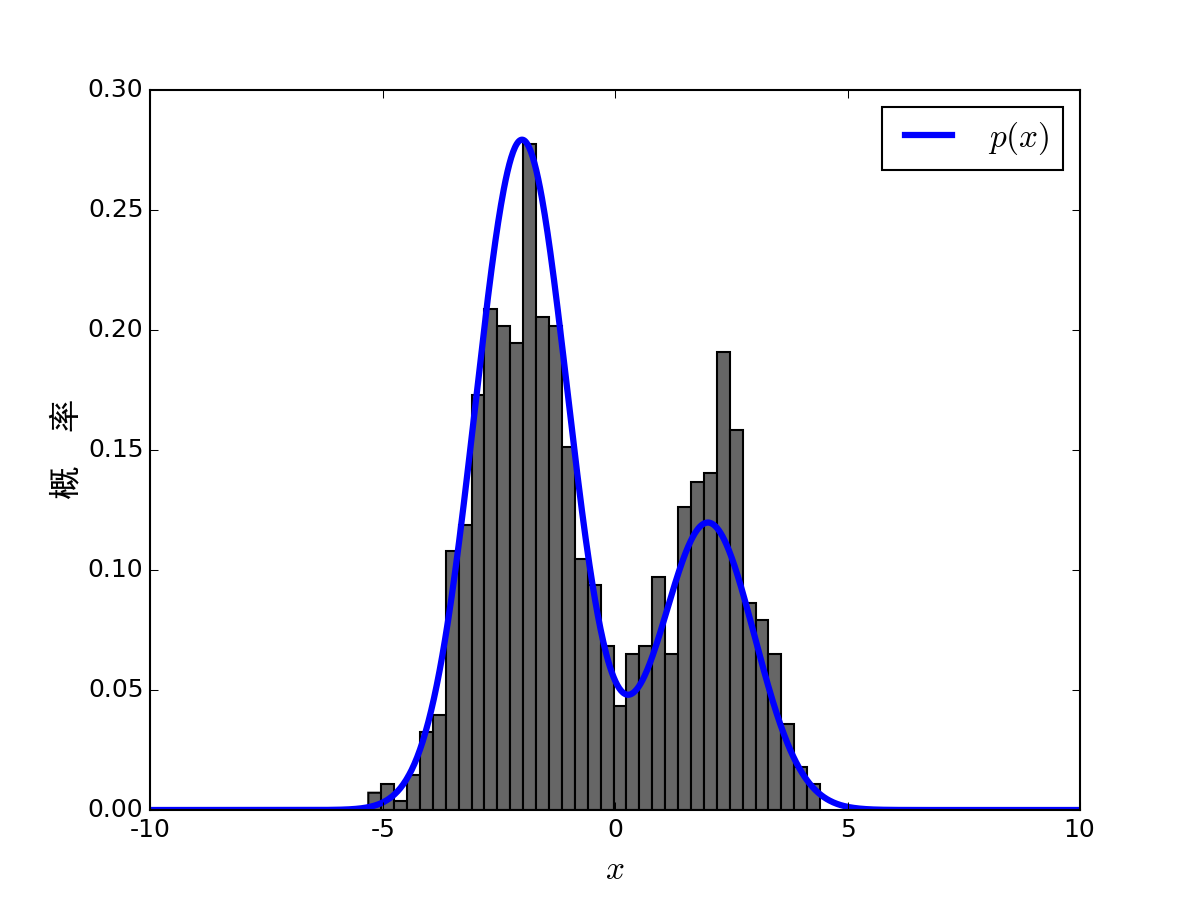
\includegraphics[width=0.4\textwidth]{MCMC/MH10.eps}}}
\subfigure{}\addtocounter{subfigure}{-2}
\subfigure{\subfigure[$N=100$]
			{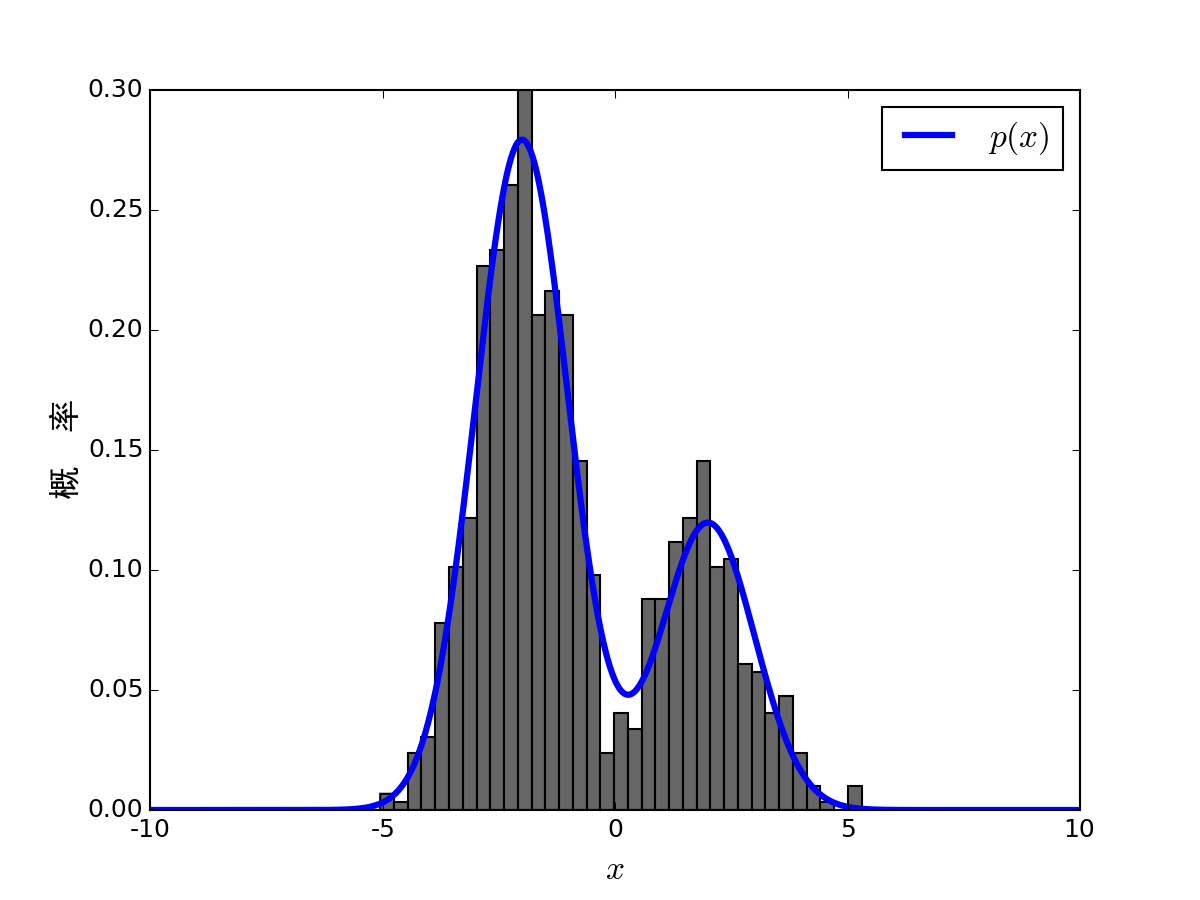
\includegraphics[width=0.4\textwidth]{MCMC/MH100.eps}}}
\subfigure{}\addtocounter{subfigure}{-2}
\subfigure{\subfigure[$N=1000$]
			{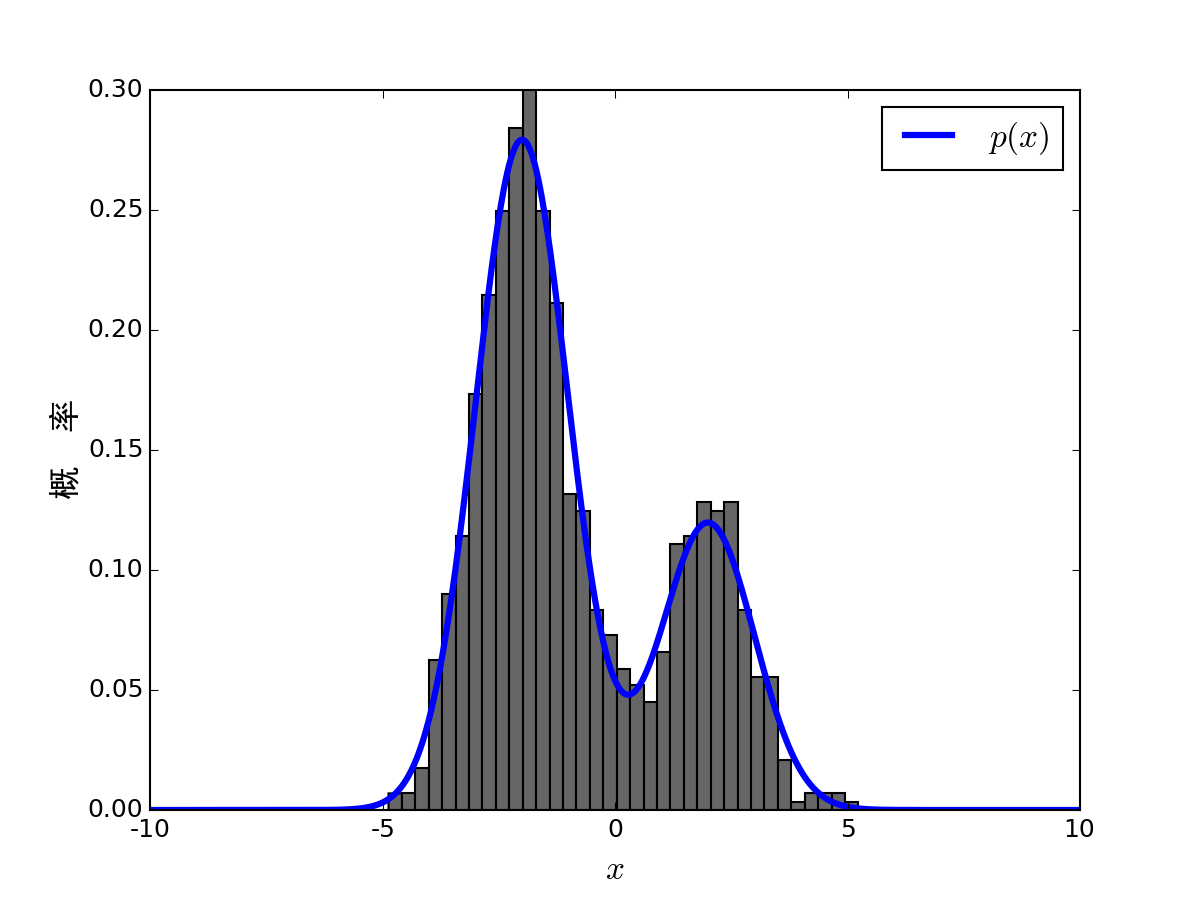
\includegraphics[width=0.4\textwidth]{MCMC/MH1000.eps}}}
			\subfigure{}\addtocounter{subfigure}{-2}
\subfigure{\subfigure[$N=100$]
			{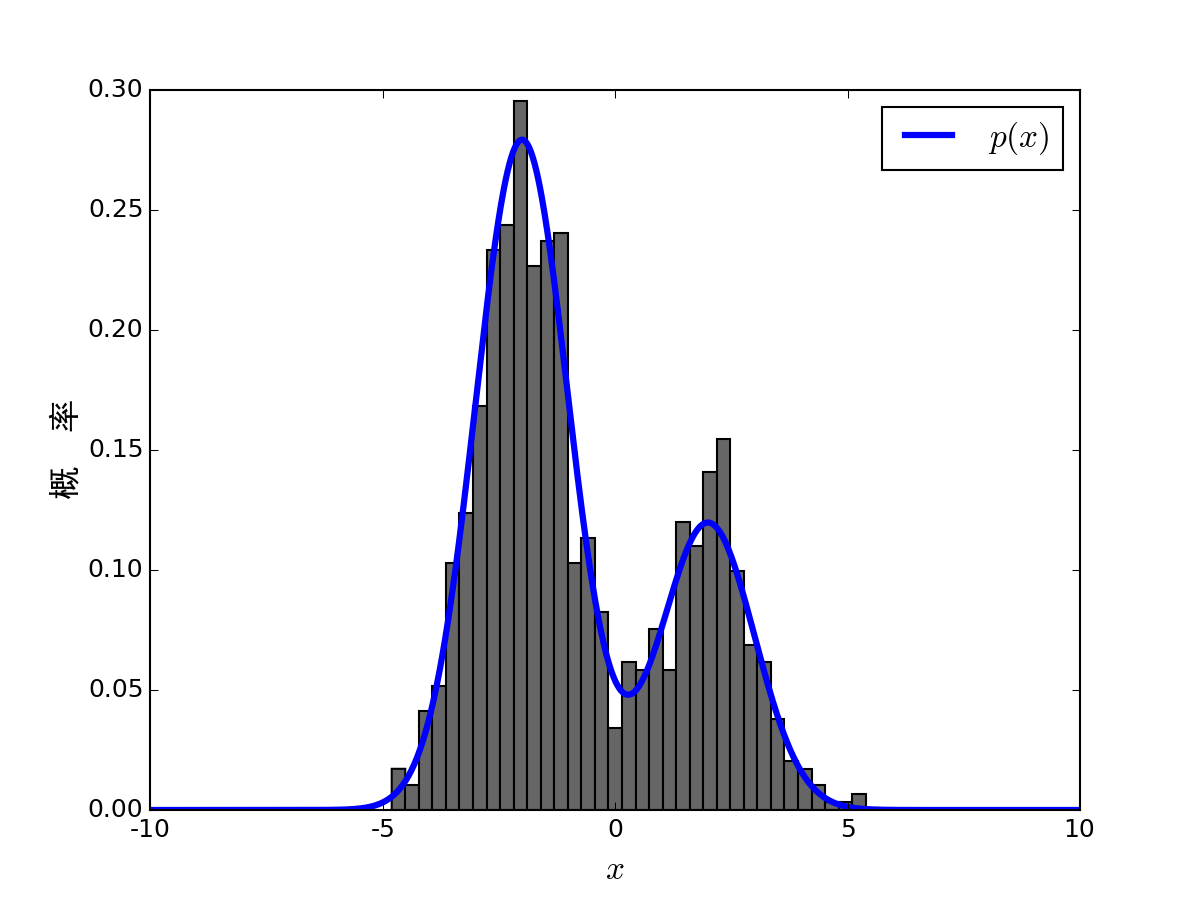
\includegraphics[width=0.4\textwidth]{MCMC/MH5000.eps}}}
\caption{不同游走次数下的样本分布直方图}
\label{img:MH}
\vspace{-1em}
\end{figure}

从图中我们不难发现,在游走次数$N=10$是,逼近效果并不完美,随着$N$的增大,当$N=100$时,采样结果已经能很好地刻画实际分布了。此时,$N$再增大(比如1000或5000)已经差别不大了。从随机游走的角度上看,可以理解为,$N=100$时就已经进入平稳分布了,再继续游走下去并没有太大意义。

MH采样可以认为是很多MCMC方法的模板,其他的MCMC方法大多都是MH算法的特例。之所以会从MH算法中衍生出这么多的分支是因为MH有其自身的局限性。首先,我们难以估计状态是否进入平稳状态,即游走次数$N$难以确定。其次,MH算法在高维问题中的效果并不好,因为高维空间的地形复杂,MH算法一不小心就会落入一个周围状态的接受概率都很小的区域,这将导致试探状态不断地被否决,从而长时间留滞在该点附近。接受概率的存在,使得游走效率低下,而Gibbs采样时MH采样的一个特例,这种方法不存在接受概率,或者说接受概率为1,因此每一次游走都将得到一个新的状态,这个特性将大大地加快收敛速度。

\BiSection{Gibbs采样}
xGibbs采样又称为热浴方法或“Glaber动力学”,常用于解决高维分布中的采样问题。假设我们有一个$d$维向量$x$,并且知道任一分量的条件概率分布形式
\begin{equation}
p(x_j|x_{-j}) \triangleq p(x_j|x_1, \cdots, x_{j-1}, x_{j+1}, \cdots x_d)
\end{equation}
则我们构建提议分布
\begin{equation}\label{equ:GibbsQx}
q(x^*|x) = \left\{
\begin{array}{cc}
p(x^*_j|x_{-j}) & \text{若} x^*_{-j} = x_{-j}\\
0 & \text{其他}
\end{array}
\right.
\end{equation}

由于Gibbs采样是MH采样的特例,而MH采样的接受概率公式\eqref{equ:MHaccept}又可以描述为
\begin{equation}\label{equ:MHaccept2}
A = \min\Big\{1, \frac{p(x^*)\cdot q(x|x^*)}{p(x)\cdot q(x^*|x)} \Big\}
\end{equation}
将式\eqref{equ:GibbsQx}代入式\eqref{equ:MHaccept2},并利用$x^*_{-j} = x_{-j}$性质以及贝叶斯公式,有
\begin{equation}\label{equ:GibbsAccept}
\begin{split}
A &= \min\bigg\{1, \frac{p(x^*)\cdot p(x_j|x^*_{-j})}{p(x)\cdot p(x^*_j|x_{-j})} \bigg\}\\
&=\min\bigg\{1, \frac{p(x^*)\cdot p(x_j|x_{-j})}{p(x)\cdot p(x^*_j|x^*_{-j})} \bigg\}\\
&=\min\bigg\{1, \frac{p(x_{-j})}{p(x^*_{-j})} \bigg\}\\
&=1
\end{split}
\end{equation}

由式\eqref{equ:GibbsAccept}我们不难得出结论,Gibbs的接受概率恒为1,亦即在Gibbs采样中,我们不存在丢弃样本或状态停滞的行为,每一次都会转移到一个新的状态上,这显然会加快算法的收敛速度。

以上内容未免过于晦涩,为了方便大家理解,我们将再次阐述Gibbs采样的原理。首先,Gibbs采样要基于一个大前提---真实分布$p(x)$在各个维度的条件概率分布是已知的,即$p(x_j|x_1,\cdots, x_{j-1}, x_{j+1}, \cdots, x_d)$已知。如果这个条件概率分布是未知的,则使用Gibbs采样不是一个恰当的策略,应为Gibbs采样的提议分布是基于这个条件概率分布之上构建出来的。式\eqref{equ:GibbsQx}定义的提议分布,其含义为:固定$x_1,\cdots, x_{j-1}, x_{j+1}, \cdots, x_d$这$d-1$个维度的状态不变,单独处理$d$个维度中的一个,即$x_j$。如果将Gibbs采样试想成为一只章鱼,那么每次它都只迈出一只脚,当这只脚固定后,再迈出剩下的另一只脚,因此,Gibbs采样的算法描述如算法所示。

\vspace{1em}
\begin{minipage}{0.8\textwidth}\centering
\begin{algorithm}[H]\label{alg:Gibbs}
 \caption{Gibbs采样算法}
  \KwIn{各个维度的条件分布$p(x_j|x_{-j})$; 游走次数$N$}
 \KwOut{$1$个采样样本$x^{(N)}$}
设置初始状态$x^{(0)}$,$i=0$\;
\Repeat{$i=N$}
{
采样出第1个维度$x_1^{(i+1)} \sim p(x_1|x_2^{(i)}, x_3^{(i)}, \cdots, x_d^{(i)})$\\
采样出第2个维度$x_2^{(i+1)} \sim p(x_2|x_1^{(i+1)}, x_3^{(i)}, \cdots, x_d^{(i)})$\\
~~~~~~~~~~~~~~~~~~~~~~~~~~~~~~~~~~~~~~~~$\vdots$\\
采样出第$j$个维度$x_j^{(i+1)} \sim p(x_j|x_1^{(i+1)},  \cdots, x_{j-1}^{(i+1)}, x_{j+1}^{(i)}, x_d^{(i)})$\\
~~~~~~~~~~~~~~~~~~~~~~~~~~~~~~~~~~~~~~~~$\vdots$\\
采样出第$d$个维度$x_d^{(i+1)} \sim p(x_d|x_1^{(i+1)}, x_2^{(i+1)}, \cdots, x_{d-1}^{(i+1)})$\\
}
返回$x^{(N)}$
\end{algorithm}
\end{minipage}
\vspace{1em}

至此,MCMC的大体内容已讨论完毕,让我们回到第\ref{chapter:RBM}章遗留的问题。第\ref{chapter:RBM}章中,式\eqref{expectFunc},即
\begin{equation}
 \frac{\partial\ln\mathcal{L}_{\hat{v}} }{\partial\theta} =  
 -\mathbb{E}_{p(h|\hat{v})}\bigg[ \frac{\partial E(\hat{v}, h)}{\partial \theta} \bigg]
 + \mathbb{E}_{p(v, h)}\bigg[\frac{\partial E(v, h)}{\partial \theta}\bigg]
\end{equation}
我们说,式中的第一项期望是容易处理的,而第二项却难以处理,因为如果我们采用穷举的方法解决这个问题,这将会是一个$O(2^{n_v+n_h})$复杂度的运算,但采用MCMC的方法就很好处理。由于目前我们需要解决的问题是$\frac{\partial E(v, h)}{\partial \theta}$在分布$p(v, h)$下的期望,根据式\eqref{eq:RBMenergy}中对能量函数$E(v,h)$的定义,偏导数非常容易求取。如果我们能在$p(v, h)$中采样出多个样本,那么这个问题便迎刃而解。但采样$p(v,h)$是一件困难的事,幸运的是,我们知道$p(v,h)$的条件概率$p(v|h)$以及$p(h|v)$,即式\eqref{p(h|v)}和式\eqref{p(v|h)},因此我们完全可以通过Gibbs采样,经过多次状态转移后采样出一个样本,再以同样的方法采样出多个样本,利用这多个样本,加以式\eqref{equ:MCintProx},便可以算出期望值,整个问题便解决了。

\BiSection{对比离差}
x尽管第\ref{chapter:RBM}章遗留的问题可以通过Gibbs采样解决,但事实上,正如我们前面提及到的,马尔可夫链进入平稳分布的时间难以确定。我们知道,马尔可夫链的初始状态对平稳分布在性质上是没有影响的,但是不同的初始状态会影响进入平稳分布的时间。就如同往汤里加盐,在不同的位置撒下并不会影响最后的咸淡,但会影响盐在水中的扩散速度,Gibbs采样也同理,不同的初始值对收敛速度有影响。如果初始值随机设置,则模型的训练速度十分缓慢。Hinton提出了一种名为对比离差\citeup{onCDlearn}(Contrastive Divergence,简写为CD)的方法,其中心思想是:既然数据出现了,那么说明这个数据是接近于平稳分布的,因此我们令初始值为该数据样本,进行吉布斯采样,所以,对比离差算法如算法\ref{alg:CD-k}所示。

\vspace{1em}
\begin{minipage}{0.8\textwidth}\centering
\begin{algorithm}[H]\label{alg:CD-k}
 \caption{CD-k算法}
  \KwIn{条件分布$p(h|v)$和$p(v|h)$; 迭代次数$k$}
 \KwOut{$1$个采样样本$v^{(k)}$}
设置初始状态$x^{(0)}=data$,$i=0$\;
\Repeat{$i=k$}
{
采样出$h^{(i)} \sim P(h|v^{(i)})$\\
采样出$v^{(i+1)} \sim P(v|h^{(i)})$\\
}
返回$v^{(k)}$
\end{algorithm}
\end{minipage}
\vspace{1em}

算法\ref{alg:CD-k}也被称为CD-k算法,随着k的增大,采样得到的样本越接近于模型的平稳分布,但在实验中,$k=1$的时候已经能获得很不错的结果,因此我们往往令$k=1$。而得到最终的采样样本$v^{(k)}$后,对数似然的梯度近似为
\begin{equation}
\frac{\partial\ln P(v)}{\partial w_{i, j}} \approx
 P(h_i = 1 | v^{(0)})v_j^{(0)} - P(h_i = 1 | v^{(k)})v_j^{(k)}
 \label{equ:MAMAMA}
\end{equation}

\begin{equation}
\frac{\partial\ln P(v)}{\partial b_{vi}} \approx
v_j^{(0)} - v_j^{(k)}
\label{equ:MBMBMB}
\end{equation}

\begin{equation}
\frac{\partial\ln P(v)}{\partial b_{i}} \approx
 P(h_i = 1 | v^{(0)}) - P(h_i = 1 | v^{(k)})
 \label{equ:MCMCMC}
\end{equation}

CD-k算法可以认为是利用
\begin{equation}
CD_k = -\sum\limits_{h}P(h|v^{(0)})\frac{\partial E(v^{(0)} , h)}{\partial \theta} + \sum\limits_{h}P(h|v^{(k)})\frac{\partial E(v^{(k)} , h)}{\partial \theta}
\end{equation}
来近似\citeup{approximations}
\begin{equation}
\frac{\partial P(v)}{\partial \theta} = -\sum\limits_{h}P(h|v^{(0)})\frac{\partial E(v^{(0)} , h)}{\partial \theta} + \sum\limits_{v, h}P(v, h)\frac{\partial E(v , h)}{\partial \theta}
\end{equation}
利用CD-k,可以很高效地求得参数的增量$\Delta W$、$\Delta b_v$以及$\Delta b_h$,从而训练受限玻尔兹曼机来刻画数据的分布。


\BiSection{本章小结}
x本章从蒙特卡罗的核心思想说起,引入舍弃采样,由于舍弃采样的提议分布受到一个约束,为此我们又引入重要性采样。无论是重要性采样或是舍弃采样,都属于非关联采样,因此我们引入马尔可夫链,得到一个关联采样方法,即MH采样。MH采样在高维空间中效果并不好,且存在接受概率使算法效率较低,为此我们引入用于解决高维问题且不存在接受概率的Gibbs采样,通过Gibbs采样可以第\ref{chapter:RBM}章的期望问题,但Gibbs的收敛速度依赖于初始值的设定,为了选取一个较好的初始值,也为了加快算法的收敛速度,我们引入了对比离差方法。通过对比离差,可以高效的解决第\ref{chapter:RBM}章中的期望问题。事实上,马尔可夫链蒙特卡罗方法其潜力并不仅局限于此,这套方法在机器学习中还有更为广泛的应用,然而我们并没有涉及。至此,受限玻尔兹曼机的内容讨论完毕,通过一个训练好的RBM,就可以刻画数据的分布。但目前的讨论并没有进入到核心内容,我们仍没有讨论识别,或者说分类问题。在第\ref{chapter:DBN}章中,我们将介绍如何用多个RBM作为砖块垒出一个深度置信网络,并用这个网络进行图像识别。









